\documentclass[10pt,aspectratio=169]{beamer}
%\documentclass[12pt,aspectratio=169]{beamer}

%\mode<presentation>

\usepackage{natbib}
\usepackage{bibentry}
\bibliographystyle{plain}

\usepackage{graphicx}
\usepackage{breqn}
\usepackage{bm}
\usepackage{color}
\usepackage{tabularx}

\usepackage{listings}
\lstset{language=C++}

\usepackage{mathtools}
\DeclarePairedDelimiter\ceil{\lceil}{\rceil}
\DeclarePairedDelimiter\floor{\lfloor}{\rfloor}

\usepackage{animate}

\definecolor{radeonruby}{rgb}{0.87, 0, 0.19}


\usepackage{listings}



%\usepackage[utf8]{inputenc}
\definecolor{bluekeywords}{rgb}{0.63, 0.79, 0.95}
\definecolor{greencomments}{rgb}{0,0.5,0}
\definecolor{redstrings}{rgb}{0.64,0.08,0.08}
\definecolor{xmlcomments}{rgb}{0.5,0.5,0.5}
\definecolor{types}{rgb}{0.17,0.57,0.68}
\lstset{language=C++,
captionpos=b,
%numbers=left,
%numberstyle=\tiny,
frame=single,
showspaces=false,
showtabs=false,
breaklines=true,
showstringspaces=false,
breakatwhitespace=true,
escapeinside={(*@}{@*)},
commentstyle=\color{greencomments},
morekeywords={partial, var, value, get, set},
keywordstyle=\color{bluekeywords},
stringstyle=\color{redstrings},
basicstyle=\ttfamily\small,
}

\usepackage[yyyymmdd]{datetime}
\renewcommand{\dateseparator}{--}

%\usepackage[inline]{asymptote}
\usepackage{asymptote}
\def\asylatexdir{}
\def\asydir{}

\renewcommand{\thefootnote}{\fnsymbol{footnote}}

\def\clap#1{\hbox to 0pt{\hss#1\hss}}
\def\mathllap{\mathpalette\mathllapinternal}
\def\mathrlap{\mathpalette\mathrlapinternal}
\def\mathclap{\mathpalette\mathclapinternal}
\def\mathllapinternal#1#2{\llap{$\mathsurround=0pt#1{#2}$}}
\def\mathrlapinternal#1#2{\rlap{$\mathsurround=0pt#1{#2}$}}
\def\mathclapinternal#1#2{\clap{$\mathsurround=0pt#1{#2}$}}

\def\p{\pause}

\def\({\left(}
\def\){\right)}
\def\[{\left[}
\def\]{\right]}

\def\no#1{\nobreak{#1}} % stop equation breaking in dmath

\begin{asydef}
  // Global Asymptote definitions can be put here.
  import three;
  usepackage("bm");
  texpreamble("\def\V#1{\bm{#1}}");
  // One can globally override the default toolbar settings here:
  // settings.toolbar=true;
\end{asydef}

%\useinnertheme{rectangles} %specifies itemize points to be rectangles
\useoutertheme{default}

\definecolor{darkgreen}{RGB}{0, 100, 0}
\definecolor{brightpurple}{RGB}{160,32,240}

% fg specifies foreground color
% bg specifies background color
% the notation color!x!white mixes the color with 1-x amount of white
%\setbeamercolor{frametitle}{fg=darkgreen!90!black, bg=darkgreen!10!white}
\setbeamercolor{normal text}{fg=white,bg=black}
% defines color of structure elements, e.g., color of text in the
% outline, block titles many more definitions possible. Each element
% predefined by the theme can be overwritten individually

\setbeamerfont{author}{size=\small,series=\bfseries,parent=structure}

\setbeamercolor{background canvas}{bg=white}
%% \usebackgroundtemplate
%% {
%%   
\includegraphics[width=\paperwidth,height=\paperheight]{gpu_background_black.png}
%% }
\pgfdeclareimage[width=\paperwidth]{mybackground}{title.png}
\setbeamertemplate{title page}{
  \begin{picture}(0,0)
    \put(-30,-163){%
      \pgfuseimage{mybackground}
    }
    \put(250,-70){%
      \begin{minipage}[b][45mm][t]{226mm}
        \usebeamerfont{title}{\inserttitle\par}
        \ifx\insertsubtitle\@empty%
        \else%
        {\vskip0.25em%
        \usebeamerfont{subtitle}\usebeamercolor[fg]{subtitle}\insertsubtitle\par}%
        \fi%
        \vskip1cm%              
        \usebeamerfont{author}{\insertauthor\par}
        \usebeamerfont{date}\url{malcolm.roberts@amd.com}\par
        \usebeamerfont{date}\insertdate
      \end{minipage}
    }
  \end{picture}
}

%------------------------------------------------------------------------
%------------------------------------------------------------------------



\def\thetitle{Multi-GPU rocFFT}
\def\thesubtitle{Planning}
\def\theauthor{rocFFT group}
\def\theauthorinstitute{AMD}

\def\presdate{\today}

\hypersetup{
  pdftitle=\thetitle{} \thesubtitle{},
  pdfauthor=\theauthor{}
}

\title{\thetitle{}}
\subtitle{\thesubtitle{}}
\author{\theauthor{}}
\institute{\theauthorinstitute}
\date{\presdate}

\setbeamertemplate{frametitle}[default][center]
%\setbeamertemplate{footline}[frame number]
\setbeamertemplate{navigation symbols}{} 

\begin{document}

\nobibliography{../refs.bib}

\setbeamertemplate{headline}{}
%\setbeamertemplate{footline}{}

{
  \setbeamercolor{background canvas}{bg=black}
  \setbeamercolor{normal text}{fg=white,bg=black}
  \setbeamercolor{frametitle}{fg=white}
  \setbeamercolor{title}{fg=white}
  \setbeamercolor{alerted text}{fg=white}
  \setbeamercolor{structure}{fg=white}
  \usebeamercolor[fg]{normal text}
  \begin{frame}
    \titlepage
  \end{frame}
}


\setbeamercolor{normal text}{fg=black,bg=white}
\usebeamercolor[fg]{normal text}

\newcolumntype{R}{>{\raggedleft\arraybackslash}X}
\setbeamertemplate{footline}{
   \leavevmode%
   \hbox{%
     \begin{beamercolorbox}[wd=\paperwidth,ht=1ex,dp=1.125ex]{author in head/foot}%
  \begin{tabularx}{\paperwidth}{lR}
    \hfill\insertframenumber/\inserttotalframenumber\hfill\phantom{.}%
    & %
    
\includegraphics[width=0.05\textwidth]{../talks/siampp20/footerlogo} \textcolor{black}{Together We Advance\begin{animateinline}[autoplay,loop]{1}{\_}\newframe\end{animateinline}}%
    \\%
  \end{tabularx}%
  \end{beamercolorbox}%
  }%
}




\begin{frame}
  \frametitle{\thetitle{}: \thesubtitle{}}

  \begin{itemize}
  \item Use cases
  \item Comparable implementations
  \item API proposal
    \begin{itemize}
    \item Spectral Ops
    \item Multi-GPU
    \item Sparsity
    \end{itemize}
  \item Current status
  \item Opportunities
  \item Risks
  \item Plan
  \end{itemize}
  
\end{frame}

\begin{frame}
  \frametitle{Use cases}

  \bigskip

  Multi-gpu FFTs are used for simulations:
  \begin{itemize}
  \item Molecular Dynamics (MD)
    \begin{itemize}
    \item eg: NAMD, Gromacs, LAMMPS
    \item Ewald sum for electrostatic interactions
    \item Smaller portion of total runtime ($\approx 15-20\%$)
    \item Synchronization point; everyone is waiting for the FFT
    \end{itemize}
  \item Fluid solvers
    \begin{itemize}
    \item eg: HACC, GESTS
    \item FFT is used for the source term in evolution equation
    \item Most expensive part of runtime
    \end{itemize}
  \end{itemize}

\end{frame}

\begin{frame}
  \frametitle{Use cases}

  Use cases tend to be:
  \begin{itemize}
  \item Convolutions (whether the app developers know it or not)
  \item Sparsity may be present
  \item Data decomposition may not be regular
  \item Scaling is important
  \end{itemize}
  
\end{frame}


\begin{frame}
  \frametitle{Comparable implementation}


  \begin{itemize}
  \item cuFFTMp: main competitor
  \item heFFTe: open-source: performance isn't great
  \item Application-specific implementations
    \begin{itemize}
    \item Many applications (eg GESTS) have their own multi-gpu back-end
    \end{itemize}
  \item SpFFT \href{https://github.com/eth-cscs/SpFFT}{eth-cscs/SpFFT}
  \end{itemize}
  
\end{frame}


\begin{frame}
  \frametitle{API proposal}

  Multi-GPU transforms will require a rocFFT API change

  \medskip

  This should be compatible with other new features:
  \begin{itemize}
  \item Single-process multi-gpu
  \item Multi-process multi-gpu
  \item Fused operations (spectral ops)
  \item Block-level sparse data
  \end{itemize}


\end{frame}

\begin{frame}
  \frametitle{API proposal}

  \begin{center}
    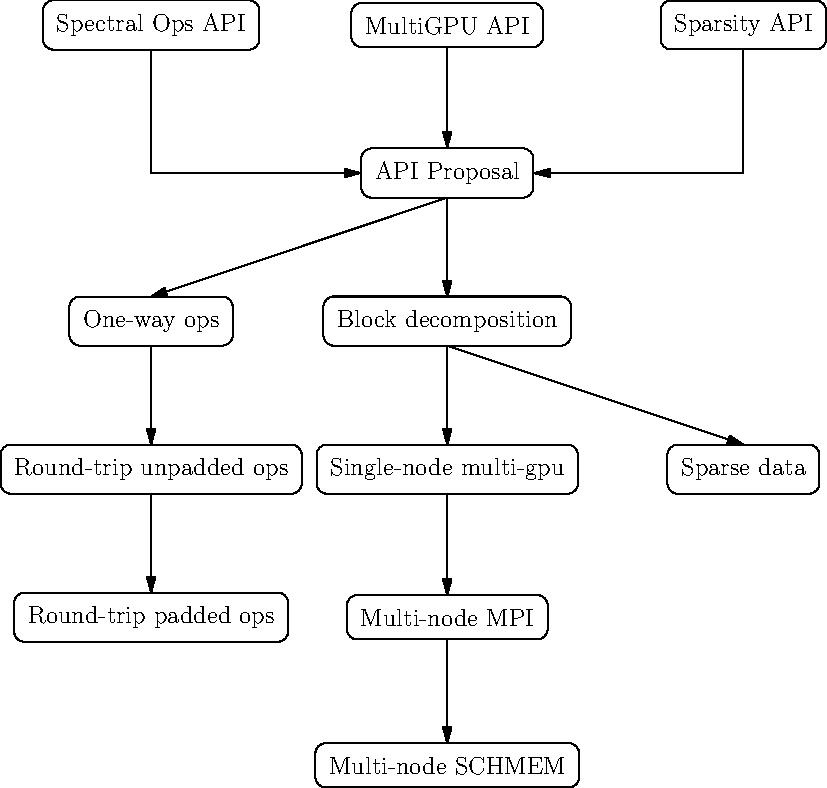
\includegraphics[width=0.9\textwidth]{implementdag.pdf}
  \end{center}
  
\end{frame}

\begin{frame}
  \frametitle{Current Status}

  \begin{itemize}
  \item We have an API design for rocFFT
  \item We are developing and API design for hipFFT
  \item Single-process multi-gpu started
    \begin{itemize}
    \item Functional implementation: ROCm 6.0
    \item Complex-complex support; no real/complex support
    \item Limited test coverage
    \item cuFFTXt behaviour needs to be reverse-engineered
    \item TODO: performance, real/complex, improve testing
    \end{itemize}
  \end{itemize}
  
\end{frame}

\begin{frame}
  \frametitle{Opportunities}

  \begin{itemize}
  \item Unified rocFFT interface
  \item Spectral Operations
  \item Sparsity and compression
  \item Algorithmic Performance Increases
  \item rocSHMEM cooperation and development
  \item Tight coupling between 1D FFTs and communication
  \end{itemize}
  
\end{frame}
  
\begin{frame}
  \frametitle{Opportunities}

  \begin{center}
    Opportunity: Unified rocFFT interface
  \end{center}
  \begin{itemize}
  \item cuFFT has very different single/multi-proc interfaces
  \item rocFFT will have a unified interface
    \begin{itemize}
    \item Multiple devices per rank
    \item Same data decomposition for single/multi proc
    \end{itemize}
  \end{itemize}

  
\end{frame}
  
\begin{frame}
  \frametitle{Opportunities}

  \begin{center}
    Opportunity: Spectral ops
  \end{center}
  \begin{itemize}
  \item People use the Fourier transform to enable other operations
  \item We can provide an interface to fuse these operations
  \item cufftDx provides somewhat analogous functionality
    \begin{itemize}
    \item limited functionality
    \item difficult to use
    \end{itemize}
  \end{itemize}

 
\end{frame}
  
\begin{frame}
  \frametitle{Opportunities}
  
  \begin{center}
    Opportunity: Sparsity and compression
  \end{center}
  \begin{itemize}
  \item Many applications seem to have a block-level sparsity
  \item We can use the brick-decomposition to mark a region as all-zero
  \item We can leverage lossless and lossy compression in the API
  \end{itemize}

  \medskip
  \begin{center}
    Opportunity: Algorithmic Performance Increases
  \end{center}
  \begin{itemize}
  \item Recursive transpose for highly decimated multi-proc FFTs
  \item Implicitly dealiased convolutions
  \item Partial-pass in off-direction may allow better communication
  \end{itemize}

 
\end{frame}
  
\begin{frame}
  \frametitle{Opportunities}

  \begin{center}
    Opportunity: coupling between 1D FFTs and communication
  \end{center}
  \begin{itemize}
  \item 
  \end{itemize}

  
  \medskip
  \begin{center}
    Opportunity: rocSHMEM development
  \end{center}
  \begin{itemize}
  \item Working with the rocSHMEM team to create a business case
  \end{itemize}

\end{frame}

\begin{frame}
  \frametitle{Risks}

  \begin{itemize}
  \item Preview and release procedure
  \item Performance requirements
  \item Single-gpu performance
  \item rocSHMEM not productized
  \item OneAPI
  \end{itemize}

\end{frame}

\begin{frame}
  \frametitle{Risks}

  \begin{center}
    Preview and release procedure
  \end{center}
  \begin{itemize}
  \item cuFFTMp had an early-access release
  \item We just push stuff to github
  \item It will take time to get everything working well
  \item What is the end-user experience during development?
  \end{itemize}

\end{frame}

\begin{frame}
  \frametitle{Risks}

  \begin{center}
    Risk: Performance requirements
  \end{center}
  \begin{itemize}
  \item If we don't get competitive performance, we lose
  \item heFFTe speed is a minimal baseline
  \item We already have prototypes with a 20\% speedup
  \item Further improvements:
    \begin{itemize}
    \item efficient buffer packing should be worth $\approx{}30\%$
    \item Recursive transpose should be effective at scale
    \item rocSHMEM should offer further improvements
    \end{itemize}
  \item It is hard to scale up to 37,888 MI250Xs
  \end{itemize}

\end{frame}

\begin{frame}
  \frametitle{Risks}

  \begin{center}
    Risk: Single-gpu performance
  \end{center}
  \begin{itemize}
  \item cuFFT has better performance than rocFFT
  \item rocFFT performance is steadily improving
    \begin{itemize}
    \item 13$x$ improvement for targeted cases (baseline: ROCm 4.0)
    \end{itemize}
  \item \emph{MI200 offered no performance uplift for rocFFT}
  \item MI300 looks better
  \end{itemize}

\end{frame}


\begin{frame}
  \frametitle{Risks}

  \begin{center}
    Risk: rocSHMEM not productized
  \end{center}
  \begin{itemize}
  \item cuFFTMp uses nvSHMEM; we would like to use rocSHMEM
  \item work needs to be done to bring rocSHMEM to a full release
  \end{itemize}

  \medskip

  \begin{center}
    Risk: OneAPI
  \end{center}
  \begin{itemize}
  \item OneAPI covers CPU and GPU
  \item AMD has separate FFT libraries for GPU, CPU, and FPGA
  \item Users do not want to have to rewrite their code all of the time
  \end{itemize}

\end{frame}


\begin{frame}
  \frametitle{Proposed Plan}

  \begin{itemize}
  \item 6.0: feature-complete
    \begin{itemize}
    \item Single-proc multi-gpu complex-complex functional
    \end{itemize}
  \item 6.1
    \begin{itemize}
    \item Single-proc multi-gpu real/complex functional
    \item Improve test coverage for single-proc multi-gpu
    \item Improve performance for single-proc multi-gpu
    \end{itemize}
  \item 6.2
    \begin{itemize}
    \item Multi-proc functional
    \end{itemize}
  \item 6.3
    \begin{itemize}
    \item Improve test coverage for multi-proc
    \item Improve performance for multi-proc
    \item Begin work on spectral ops
    \end{itemize}
  \end{itemize}

  \medskip

  We may be able to offer NDA'd prototypes before releases to help
  with tenders.

  \medskip

  We are looking for feedback on the API and priorities.
  
\end{frame}

\end{document}
